\section{Graphical Design}
\label{sec:graphical_design}

Based on our analysis, we concluded that there does not seem to be a relation between the complexity of the graphics, and the impact this has on how much fun or educating a game is.
For this reason 2D graphics has been deemed sufficient for this game.
The following section will go through the design choices that has been made in terms of the different graphical interfaces of the game, along with justification for why a given choice was made. The graphical interfaces include the board, the editor and the menu.

\subsection{Board}
The board, or world map, is a hexagon consisting of hexagonal tiles.
This means that by design the entire field is hexagons in hexagons. 
A cell takes up a single tile on the board, as does the various food types a player may encounter.
Hexagons were chosen for the map, because they add further complexity to the game in terms of 'legal movements' for a cell, relative to if we had chosen squares, see \autoref{sec:designing_playing_field}.
Hexagons seemed a good design choice, it adds the structure we need as programmers, and it opens up more avenues of play for the players.
A mock-up of the board can be seen on \autoref{fig:cells_mockup}.\newline

\begin{figure}[ht]
	\centering
		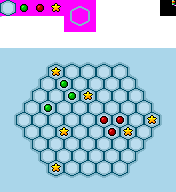
\includegraphics{img/cells_mockup.png}
	\caption{Playing field with cells and food}
	\label{fig:cells_mockup}
\end{figure}

Food in this example is a star.
We have created other mock-ups as well, such as a ham and an egg as possible alternatives. 
Cells are illustrated on the map as green and red 'balls', with green referring to a specific player's cell, and red referring to another player's cells.
This sort of green and red distinction between the players will be used all throughout the game.\todo{Anders: What does that mean? You mean the health bar?}
The icons chosen for cells and food have been chosen for the sole purpose of added clarity, that a player can within reason quickly distinct between food and their cells, and their opponents' cells.
Choosing different coloring for cells is an easy was to achieve this distinction.
With all food types taking a none-circular shape or a totally different color-scheme, such as a yellow star, it will also help the players distinct between what is food and what are actual player controlled entities.

\subsection{Health Bar}
It was decided to design a health bar at the top of the board to give the player an indication of how well he/she is doing in the game, shown on \autoref{fig:healthbar}.
The idea is that the health bar will fill with green and red colors, depending on how well the game is going for the player.
If the bar is completely green, the player has won the game, and likewise he/she will lose the game, if the bar fills with red.
The amount of red and green color is determined entirely by the total amount of energy that the players cells have in contrast to the amount of total energy the enemy cells have.
The basic idea is, that the bar will update throughout the game, sweeping back and forth depending on which player is doing best throughout a game.
\autoref{fig:healthbar} illustrates how it would look like if the green player has an advantage over the red player during the game.

\begin{figure}[ht]
	\centering
		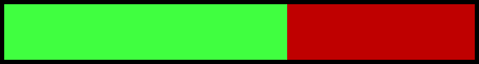
\includegraphics{img/healthbar_example.png}
	\caption{Health bar, where the player has an advantage over his opponent}
	\label{fig:healthbar}
\end{figure}

%One of the trickier parts was to work out, how is an advantage given in the game? Is it based on the number of cells a given player controls? Is it their map position on the board - for example; how many food tiles are placed on 'their territory'? Is it based on how well their algorithm functions compared to the opponent's? Ultimately we decided that it was enough to simply compare the two players' energy points, and determine who had the most energy-points.

\subsection{Menu Design}
The menu should somehow resemble the design choices that were made for the board, to make the game feel consistent.
Therefore, we have worked on a hexagonal design for our menu button and the background behind each button.
This is an early design, and the menu text may change.\newline

\begin{figure}[ht]
	\centering
		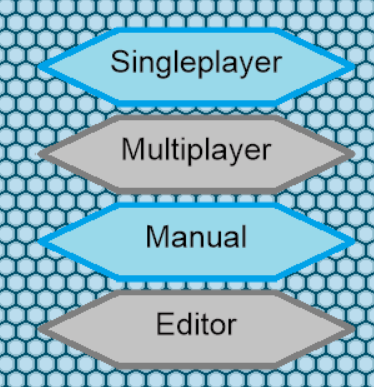
\includegraphics{img/Menu1.png}
	\caption{First menu screen the user sees}
	\label{fig:menu1}
\end{figure}

Notice the hexagonal layer in the background, which is the same kind of style used for the board.
The color scheme is the same as the board, which is a mixture of light and darker blue color. 
The options, that are not available to the user, because they will not implementing in this semester, or what the user has to unlock by completing challenges, will be drawn in a gray color scheme to symbolize inactivity.
Graying out inaccessible parts of the program seems highly used in other types of software, such as Windows, LaTeX and various video games, so the same convention will be used for this game.
Accessible options of the menu will be colored in a more vibrant, light blue, to distinct them from the gray buttons.\newline

%\begin{figure}[h]
%	\centering
%		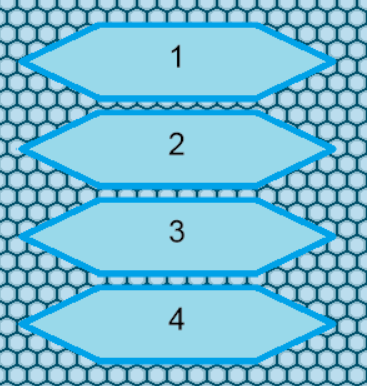
\includegraphics{img/Menu2.png}
%	\caption{Second menu screen the user sees}
%	\label{fig:menu2}
%\end{figure}

When a user clicks a menu button, a new menu will be produced.
The menu will represent potential options for the user to take, and they will follow the same color scheme as described previously.
%For examples of what these options could be under 'Singleplayer', suppose a user chooses a 'Skirmish' kind of game, in which their cell competes against a cell AI, that we have created. A user may also have access to various programming challenges, aptly named 'Challenges' in which they have to solve a puzzle - which could function as a sort of tutorial for the user to get into the program.\newline

%It is entirely possible that a menu would lead to a second, a third, and possibly a fourth.